% !TeX root = ./main.tex
\documentclass[
    a4paper,
    doc,
    % CHANGE TEXT SIZE HERE
    11pt,
]{apa6}

% to have contents as inhaltsverzeichnis and so on if localized - german example
% -> i18n babel itself get's loaded by one of the packages below
\PassOptionsToPackage{german,english}{babel}

\usepackage{csquotes}
\usepackage{fontspec}
\usepackage{polyglossia}

% DELETE IF NON GERMAN - FIXES ß character display
\setmainlanguage[babelshorthands=true]{german}

% Color page for links
\usepackage{xcolor}

% Can define other colors here
% Is good starting point
\definecolor{inner-link-blue}{rgb}{0,0,0.37}
\definecolor{cite-grey}{rgb}{0.26,0.26,0.26}
\usepackage[
    colorlinks=true, % turns of ugly boxes and sets color of links on
    linktoc=all, %table of contents links colored
    % and configure here
    linkcolor=inner-link-blue, % internal links color
    citecolor=cite-grey, % citations link color
    urlcolor={blue!80!black} % urls outside document
]{hyperref}

% to cite sources
% Other options for style,sorting available
\usepackage[sorting=none,style=apa]{biblatex}
% sources
\addbibresource{./sources.bib}

% subfiles import as last
\usepackage{subfiles}

% pictures embedding
\usepackage{graphicx}

% pdf appendix embed
\usepackage{pdfpages}

% appendix package
\usepackage[toc, page]{appendix}

% rename appendices to localize since was not done
% REMOVE IF USING ENGLISH ONLY TO LOCALIZE
\renewcommand\appendixtocname{Anhang}
\renewcommand\appendixpagename{Anhang}

% for biliography in toc
% REMOVE IF USING ENGLISH ONLY TO LOCALIZE
\DefineBibliographyStrings{german}{
    bibliography = {Referenzen},
}

% Number sections into second level for toc
% first level is section so give everything up to subsubsection numbers
\setcounter{secnumdepth}{3} % can also reduce or increase

% for some fancy tabbing modifiers and so on needed
% \usepackage[parfill]{parskip}

\title{
    My awesome paper \newline
    Lorem Ipsum
}
\shorttitle{My awesome paper – Lorem Ipsum}
\author{Max Mustermann – Group 1337}
\affiliation{Julius-Maximilians Universität}
% \date{Februar 2020}

\keywords{keywordOne,lorem,ipsum}

% able to cut down to page limits with this margin trick
% especially thick 2.5cm bottom margin can be reduced
%\geometry{bottom=1.7cm}
% possible values: left,right,bottom,top,hmargin,vmargin
% accepts centimeters as cm and inches as in

% thanks https://tex.stackexchange.com/a/483040
% only use this while writing on large files 
% and want to save time at compilation on save
% many images blow up size if compression is disabled here
% and if compression is enabled they blow up build time
% final pdf should be gzipped so comment out then
% \special{dvipdfmx:config z 0}

\begin{document}

\maketitle

\newpage

% disables page numbering and shorttitle show on table of content pages
% thanks to https://tex.stackexchange.com/a/2996
\addtocontents{toc}{\protect\thispagestyle{empty}}

\tableofcontents

\newpage
\setcounter{page}{1}
\section{Summary}
\subfile{sections/summary}

\newpage
\section{Section One}
\subfile{sections/sectionOne}

\newpage
% other more space efficient way to seperate sections
% \vspace*{0.5 cm}
\section{Section Two}
\subfile{sections/sectionTwo}


%%%%%%%%%%% Bilbiography %%%%%%%%%%%%%%
\newpage
% Use single whole bibliography info
% can also split into keywords for sections and print multiples
\printbibliography[heading=bibintoc]{sources}


%%%%%%%%%%% Appendices %%%%%%%%%%%%%%
\newpage
\begin{appendices}
% reset section counter to be 1 since A prefix is added automatically in appendice
% and want it to start with A-1
\setcounter{section}{1}


% Pdf appendix
\begingroup
    \centering
    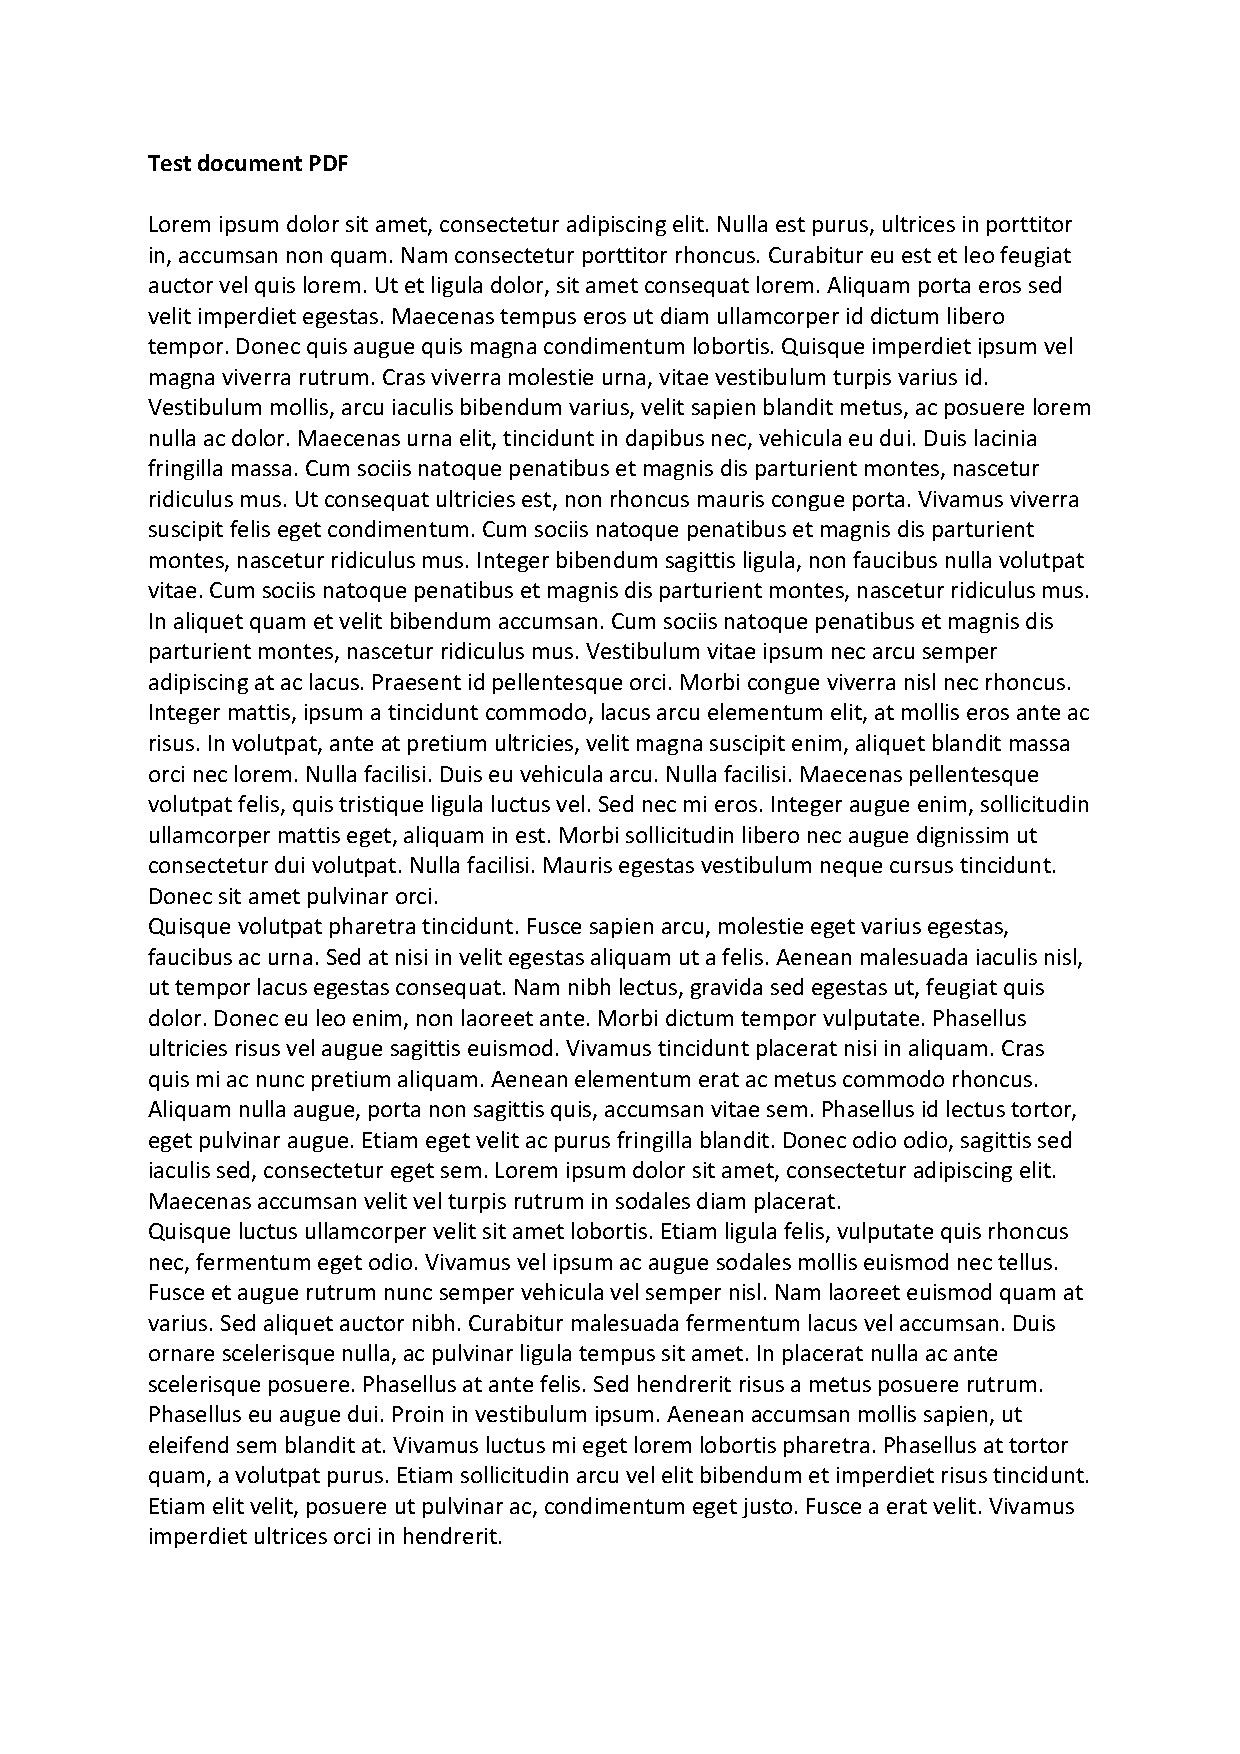
\includepdf[scale=0.85,pages={1},pagecommand=\subsection{Lorem Ipsum}]{appendix/lorem-ipsum.pdf}
    \label{append:lorem_ipsum}
    % REST OF THE PAGES AFTER FIRST WITH SAME FILE NAME HERE
    % example pdf only has one page
    % \includepdf[pages={2-}]{appendix/lorem-ipsum.pdf}
\endgroup

% Image appendix
\newpage
\subsection{Example Picture appendix}
\begingroup
    \begin{figure}[h!]
        \centering
        \label{append:pic:one}
        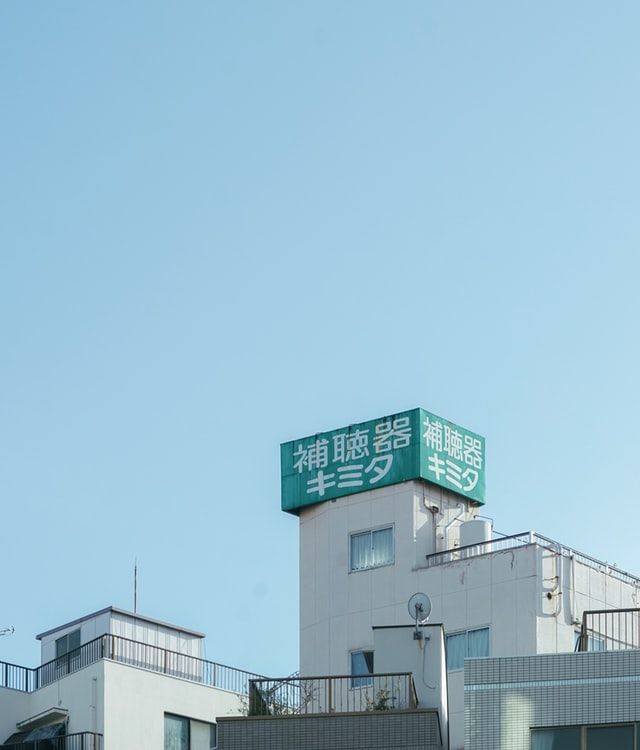
\includegraphics[width=0.9\textwidth]{appendix/imageExample/pOne.jpg}
        \caption{Image description for image One.}
    \end{figure}
    \newpage
    \begin{figure}[h!]
        \centering
        \label{append:pic:two}
        
\includegraphics[width=0.9\textwidth]{appendix/imageExample/pTwo.jpg}
        \caption{Image description for image Two.}
    \end{figure}
\endgroup

% tabel appendix
\newpage
\begingroup
\subsection{Example Table}
    \subsubsection{First table}
    \label{append:example_table}
    \begin{center}
        \begin{tabular}{ |c|c| }
            \hline
            quismagnacondimentum & Count \\
            \hline
            tinciduntindapibus & 12 \\ 
            Cumsociisnatoque & 18 \\ 
            magnisdisparturient & 5 \\ 
            ridiculusmus & 1 \\ 
            \hline
        \end{tabular}
    \end{center}
\endgroup

% Another pdf appendix
\newpage
\begingroup
    \centering
    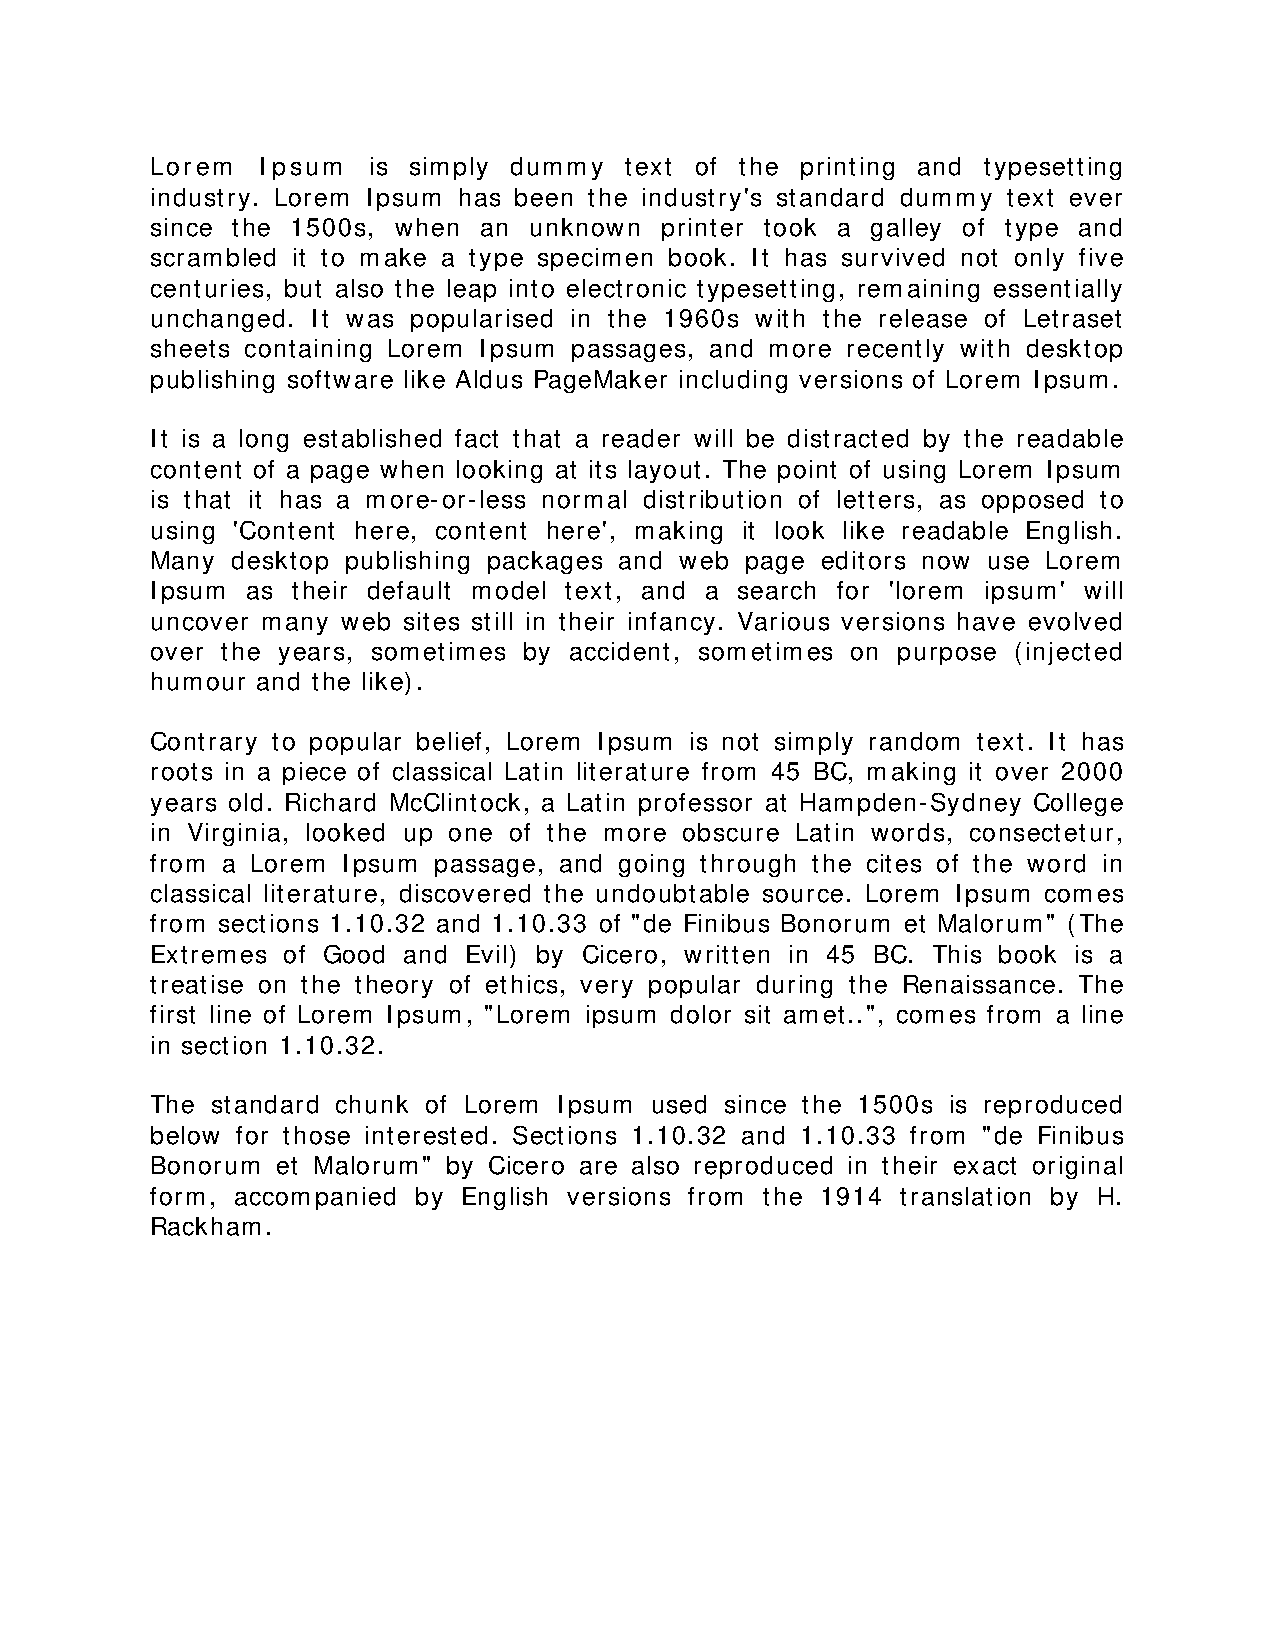
\includepdf[scale=0.8,pages={1},pagecommand=\subsection{Lorem Ipsum – Information}]{appendix/lorem-ipsum-info.pdf}
    \label{append:ipsum_info}
    % REST OF THE PAGES AFTER FIRST WITH SAME FILE NAME HERE
    % example pdf only has one page
    % \includepdf[pages={2-}]{appendix/lorem-ipsum-info.pdf}
\endgroup

\end{appendices}
\end{document}
